% Provenance (never printed): see sources/outline_sources.md (Year 2: natural hazards and risks
% quantified --- recurrence, probabilistic hazard, slope stability, tsunamis, floods, warning).
% Terminology from the UN report A/71/644 (UNDRR); the 475-year convention from the USGS
% Earthquake Hazards 201 page; the ground-motion prediction equation of Boore, Joyner and Fumal
% (USGS Open-File Report 93-509); run-ups from the NOAA NCEI tsunami database; the 1999 Vargas
% debris flows from USGS Open-File Report 01-0144. Ledger rows in sources/ledger/book4.md;
% curves and numbers from figdata/bachelor-2/hazards.py and the Book 4 second-writer scratch
% calculator calc/ch28.py. Hazards are described and quantified physically only: no advice.
\chapter{Geological Hazards and Risk}\label{ch:b2:geological-hazards}

A building designed for the ground motion that is exceeded, on average, once in 475 years has a
one-in-ten chance of meeting it during a fifty-year life. The two statements are the same number
read in two ways, and moving between them is the daily work of hazard science. This chapter
builds its tools: the probability of rare events, the \omterm{def:b2:geological-hazards:psha}{hazard curve} of a site, the stability of a
slope, the speed and the run-up of a tsunami, the frequency of floods, and the physics that sets
how much warning each hazard can give.
% ledger: usgs:eh201-475

\begin{recall}
\textbf{From the school volumes}: natural hazard, natural disaster and landslide; vulnerability,
risk, prevention and the hazard map; tsunami; the \omterm{def:b2:geological-hazards:return}{return period} of a flood, and the rank formula
$T = (n + 1)/m$ for a record of $n$ annual peaks. \textbf{From the Year 1 volume}: the
Gutenberg--Richter law $\log_{10} N(\geq M) = a - bM$ and its b-value; seismic moment and moment
magnitude; pore-fluid pressure, effective stress $\sigma' = \sigma - u$ and the Coulomb failure
criterion $\tau = c' + \sigma' \tan\varphi'$. \textbf{From \cref{ch:b2:eruptive-styles}}: \omterm{def:b2:eruptive-styles:pdc}{pyroclastic
density currents}, \omterm{def:b2:eruptive-styles:lahar}{lahars} and \omterm{def:b2:eruptive-styles:tephra}{tephra} fall. \textbf{From the mathematics books}: the Poisson and
exponential distributions, the normal distribution and its distribution function $\Phi$.
\textbf{From the physics books' Year 2 volume}: the dispersion relation of surface gravity waves,
$\omega^2 = gk\tanh(kh)$.
\end{recall}

\section{Hazard, exposure and risk}\label{sec:b2:geological-hazards:risk}

\begin{definition}[Geological hazard, exposure, disaster risk]\label{def:b2:geological-hazards:risk}
A \emph{geological hazard}\index{geological hazard} is a process or phenomenon that originates in
the internal processes of the Earth --- an earthquake, an eruption, a mass movement such as a
landslide or a \omterm{def:b2:geological-hazards:slope}{debris flow} --- and may cause loss of life, injury, damage or disruption. It is
characterised by its location, its intensity or magnitude, and its frequency or probability. The
\emph{exposure}\index{exposure (to a hazard)} to a hazard is the situation of the people,
buildings, infrastructure and other assets located where the hazard can reach, measured by their
number or their value. \emph{Disaster risk}\index{disaster risk} is the potential loss of life,
health or assets that could occur in a given period, determined probabilistically from the
hazard, the exposure and the vulnerability of what is exposed.
\end{definition}
% ledger: undrr:hazard, undrr:geological, undrr:exposure, undrr:disaster-risk, undrr:vulnerability

The international terminology classes tsunamis apart: triggered by earthquakes and other
geological events, they become an oceanic process and strike as a coastal, water-related hazard.
This chapter treats them with the others, because their source is geological.
% ledger: undrr:geological

The definition contains a product. If events of intensity $i$ occur at an annual rate
$\lambda_i$, if the exposed assets are worth $E$, and if an event of intensity $i$ destroys a
fraction $V_i$ of them (the vulnerability, between 0 and 1), the expected annual loss is
\begin{equation}
L = \sum_i \lambda_i \, E \, V_i ,
\label{eq:b2:geological-hazards:loss}
\end{equation}
often abbreviated to risk = hazard $\times$ \omterm{def:b2:geological-hazards:risk}{exposure} $\times$ vulnerability. The risk vanishes when
any factor does: a violent volcano on an empty island, a crowded city on a quiet \omterm{def:b2:precambrian-earth:craton}{craton}, or
buildings that resist the shaking. Hazard science measures the first factor; the figure below
places it among the three.

\begin{omfigure}
\centering
\begin{tikzpicture}[font=\small]
\fill[omThm!14] (90:1.05) circle (1.55);
\fill[omDef!14] (210:1.05) circle (1.55);
\fill[black!8] (330:1.05) circle (1.55);
\begin{scope}
\clip (90:1.05) circle (1.55);
\clip (210:1.05) circle (1.55);
\fill[omThm!45!omDef!45] (330:1.05) circle (1.55);
\end{scope}
\draw[omThm, thick] (90:1.05) circle (1.55);
\draw[omDef, thick] (210:1.05) circle (1.55);
\draw[black!60, thick] (330:1.05) circle (1.55);
\node[align=center, anchor=south] at (0,2.65) {\textbf{hazard} {\scriptsize (rate $\lambda_i$, intensity)}};
\node[align=right, anchor=east] at (-2.55,-1.35) {\textbf{exposure}\\[-1pt]{\scriptsize assets $E$}};
\node[align=left, anchor=west] at (2.55,-1.35) {\textbf{vulnerability}\\[-1pt]{\scriptsize fraction lost $V_i$}};
\node[align=center, font=\scriptsize\bfseries] at (0,0) {risk};
\end{tikzpicture}
\par\smallskip{\small The three factors of \omterm{def:b2:geological-hazards:risk}{disaster risk}. The expected loss is non-zero only where
all three overlap: a hazard that reaches something exposed and able to be harmed.}
\end{omfigure}

\section{The probability of rare events}\label{sec:b2:geological-hazards:probability}

\begin{definition}[Return period]\label{def:b2:geological-hazards:return}
Let events of a given kind --- a flood above a discharge, a ground motion above a level, an
earthquake above a magnitude --- occur at a mean annual rate $\lambda$. Their \emph{return
period}\index{return period} is $T = 1/\lambda$: the mean interval between two of them, and the
inverse of their annual rate, not a timetable.
\end{definition}
% ledger: usgs:eh201-475

\begin{definition}[Exceedance probability]\label{def:b2:geological-hazards:poisson}
The \emph{exceedance probability}\index{exceedance probability} of a level in an exposure time $t$
is the probability that the level is equalled or exceeded at least once during $t$.
\end{definition}

\begin{proposition}[Poisson recurrence model]\label{prop:b2:geological-hazards:poisson}
Suppose that events occur one at a time\index{Poisson recurrence model}, independently of one
another and of the time elapsed, at a constant mean rate $\lambda = 1/T$. Then the number $N$ of
events in a time $t$ follows the Poisson distribution of mean $\lambda t$; the \omterm{def:b2:geological-hazards:poisson}{exceedance
probability} in $t$ is
\begin{equation}
P(t) = 1 - e^{-t/T};
\label{eq:b2:geological-hazards:poisson}
\end{equation}
and the interval between successive events follows the exponential distribution of mean $T$.
\end{proposition}

\begin{proof}
Let $P_k(t)$ be the probability of $k$ events in $[0, t]$. In a short interval $\mathrm{d}t$ an
event occurs with probability $\lambda\,\mathrm{d}t$, independently of the past, and two with a
probability of higher order. Hence $P_0(t + \mathrm{d}t) = P_0(t)(1 - \lambda\,\mathrm{d}t)$, that is
$P_0' = -\lambda P_0$ with $P_0(0) = 1$: $P_0(t) = e^{-\lambda t}$, and $P(t) = 1 - P_0(t)$. In the
same way $P_k' = \lambda(P_{k-1} - P_k)$ for $k \geq 1$, solved by induction:
$P_k(t) = (\lambda t)^k e^{-\lambda t}/k!$, the Poisson distribution of mean $\lambda t$. Started at
an event, the same argument gives the probability that the next one comes later than $t$:
$e^{-\lambda t}$, the survival function of the exponential distribution, whose mean is
$\int_0^\infty e^{-\lambda t}\,\mathrm{d}t = 1/\lambda = T$.
\end{proof}

Two consequences are used everywhere. For a probability $p$ in an exposure time $t$, the \omterm{def:b2:geological-hazards:return}{return
period} is $T = -t/\ln(1 - p)$: \qty{10}{\percent} in 50 years gives $T = 50/0.10536 =
474.6$ years, the ``475-year'' motion of building codes, and \qty{2}{\percent} in 50 years
gives 2475 years. And when $t \ll T$, $P \approx t/T$: the rate can be read as a
probability per year. Over one full \omterm{def:b2:geological-hazards:return}{return period}, by contrast, the probability is $1 - e^{-1} =
\qty{63}{\percent}$, not 1. The figure below (left) draws \eqref{eq:b2:geological-hazards:poisson}
for three \omterm{def:b2:geological-hazards:return}{return periods}.
% ledger: usgs:eh201-475
% values: T 474.561 and 2474.92 years; P(50|475) 0.0999 (hazards.py numbers)

Is the model true? The global catalogue of earthquakes of magnitude at least 7 holds 696 events
from 1976 to 2025, 695 intervals with a mean of 26.2 days. If they were a Poisson process,
the fraction of intervals longer than $t$ would be $e^{-t/26.2}$, a straight line on a logarithmic
axis. The figure below (right) shows that it nearly is: \qty{30.4}{\percent} of the intervals are
longer than 30 days, against \qty{31.8}{\percent} for the model, and the standard deviation of the
intervals is 1.07 times their mean, against exactly 1. The defect is at short intervals: 36 pairs
fall on the same day, aftershocks and doublets that a memoryless process would not cluster. Hazard
maps therefore remove the dependent events from a catalogue, declustering it, so that the
mainshocks left can be treated as a Poisson process; their rates by magnitude come from the
Gutenberg--Richter law.
% ledger: data:usgs-comcat, usgs:eh201-poisson
% values: m7_events 696, mean 26.2245 d, cv 1.06891, same-day 36, frac>30 d 0.303597 vs 0.318552

\begin{omfigure}
\centering
\begin{minipage}[b]{0.49\linewidth}\centering
\begin{tikzpicture}
\begin{axis}[omrecord, width=0.96\linewidth, height=5.2cm, xmin=0, xmax=200, ymin=0, ymax=1,
  xlabel={exposure time $t$ (years)}, ylabel={exceedance probability},
  tick label style={font=\scriptsize}, label style={font=\small},
  xtick={0,50,100,150,200}, ytick={0,0.2,...,1}]
% computed in figdata/bachelor-2/hazards.py part poisson
\addplot[omThm, line width=1pt] table[x=t_yr, y=P50] {figdata/out/bachelor-2-hazards-poisson.dat};
\addplot[omDef, line width=1pt] table[x=t_yr, y=P475] {figdata/out/bachelor-2-hazards-poisson.dat};
\addplot[black!70, line width=1pt, densely dashed] table[x=t_yr, y=P2475] {figdata/out/bachelor-2-hazards-poisson.dat};
\draw[black!50, densely dotted] (axis cs:50,0) -- (axis cs:50,1);
\fill[omDef] (axis cs:50,0.1) circle (1.8pt);
\node[font=\scriptsize, text=omThm, anchor=west] at (axis cs:62,0.86) {$T = 50$};
\node[font=\scriptsize, text=omDef, anchor=west] at (axis cs:120,0.34) {$T = 475$};
\node[font=\scriptsize, text=black!70, anchor=west] at (axis cs:120,0.12) {$T = 2475$};
\node[font=\scriptsize, anchor=west, text=omDef] at (axis cs:52,0.2) {\qty{10}{\percent}};
\end{axis}
\end{tikzpicture}
\end{minipage}\hfill
\begin{minipage}[b]{0.49\linewidth}\centering
\begin{tikzpicture}
\begin{axis}[omrecord, width=0.93\linewidth, height=5.2cm, xmin=0, xmax=120, ymode=log,
  ymin=0.008, ymax=1.1, xlabel={interval $t$ (days)}, ylabel={fraction of intervals $> t$},
  tick label style={font=\scriptsize}, label style={font=\small}, xtick={0,30,60,90,120},
  legend style={at={(0.03,0.03)}, anchor=south west, font=\scriptsize, draw=black!30},
  legend cell align=left]
% computed in figdata/bachelor-2/hazards.py part survival; ledger: data:usgs-comcat
\addplot[omThm, only marks, mark=*, mark size=1.2pt] table[x=t_day, y=observed] {figdata/out/bachelor-2-hazards-survival.dat};
\addlegendentry{$M \geq 7$, 1976--2025}
\addplot[black, line width=0.9pt] table[x=t_day, y=poisson] {figdata/out/bachelor-2-hazards-survival.dat};
\addlegendentry{Poisson, mean 26.2 days}
\end{axis}
\end{tikzpicture}
\end{minipage}
\par\smallskip{\small Left: the probability of at least one event in an exposure time $t$ for
\omterm{def:b2:geological-hazards:return}{return periods} of 50, 475 and 2475 years; the 475-year event has a \qty{10}{\percent} chance in 50
years. Right: the intervals between the 696 earthquakes of magnitude at least 7 in the global
catalogue of 1976--2025, against the exponential law of a Poisson process of the same rate. Data:
USGS ANSS Comprehensive Catalog.}
\end{omfigure}

\section{Seismic hazard}\label{sec:b2:geological-hazards:seismic}

\begin{definition}[Probabilistic seismic hazard analysis, ground-motion prediction equation, peak ground acceleration, hazard curve]\label{def:b2:geological-hazards:psha}
The \emph{peak ground acceleration}\index{peak ground acceleration} (PGA) at a site is the largest
absolute horizontal acceleration of the ground during an earthquake, usually expressed as a
fraction of $g$. A \emph{ground-motion prediction equation}\index{ground-motion prediction
equation} (GMPE) gives the probability distribution of a measure of shaking such as the PGA at a
site --- a median and a scatter --- as a function of the magnitude, the distance to the source
and the ground conditions. \emph{Probabilistic seismic hazard analysis}\index{probabilistic
seismic hazard analysis} (PSHA) combines all the earthquakes that can affect a site, with their
rates and distances, with a GMPE, to give the annual rate at which each level of shaking is
exceeded. The curve of that rate against the level is the site's \emph{hazard
curve}\index{hazard curve}.
\end{definition}
% ledger: usgs:eh201-pga, usgs:eh201-475

The PGA is what a particle of the ground experiences. A building responds to the part of the
motion near its own natural period, and codes also map that response, the spectral acceleration;
the PGA keeps the reasoning simple and is used here.
% ledger: usgs:eh201-pga

\begin{method}[A probabilistic seismic hazard analysis]\label{met:b2:geological-hazards:psha}
\begin{enumerate}
  \item \textbf{Sources.} Map the faults and source zones around the site, and the distance $d$ of
        each to the site.
  \item \textbf{Recurrence.} For each source, take the annual rate of earthquakes by magnitude
        from a Gutenberg--Richter law, truncated at a maximum magnitude $M_{\max}$:
        $N(\geq m) = 10^{a - bm} - 10^{a - bM_{\max}}$, from a minimum magnitude $M_{\min}$.
        Cut the range into slices of rate $\nu_j$ around magnitudes $m_j$.
  \item \textbf{Ground motion.} From the GMPE, take the median $\mu_j = \log_{10}\mathrm{PGA}$ and
        the scatter $\sigma$ for each slice; the probability that the PGA exceeds $a$ is
        $1 - \Phi\bigl((\log_{10} a - \mu_j)/\sigma\bigr)$.
  \item \textbf{Sum.} The annual rate of exceedance of $a$ is $\lambda(a) = \sum_j \nu_j
        \bigl[1 - \Phi\bigl((\log_{10} a - \mu_j)/\sigma\bigr)\bigr]$, summed over all sources.
  \item \textbf{Read.} The PGA with a probability $p$ of exceedance in $t$ years is the level where
        $\lambda(a) = -\ln(1 - p)/t$: \num{2.107e-3} per year for \qty{10}{\percent} in 50 years.
\end{enumerate}
\end{method}

The GMPE used in this chapter is that of Boore, Joyner and Fumal, fitted to 271 recordings of 20
earthquakes in western North America: for a random horizontal component, in units of $g$,
\begin{equation}
\log_{10}\mathrm{PGA} = -0.105 + 0.229\,(M - 6) - 0.778\log_{10} r + 0.162\,G_B + 0.251\,G_C,
\qquad r = \sqrt{d^2 + 5.57^2},
\label{eq:b2:geological-hazards:gmpe}
\end{equation}
with $M$ the moment magnitude, $d$ the distance in kilometres to the surface projection of the
rupture, and a scatter $\sigma = 0.230$ about the median. It holds for $5.0 \leq M \leq 7.7$ and $d
\leq \qty{100}{km}$. The constant \qty{5.57}{km} is a fictitious depth fitted by the regression,
which keeps the motion finite above the source. A magnitude 6 at \qty{15}{km} gives a median of
\qty{0.091}{g}, a magnitude 7.5 \qty{0.200}{g}; one standard deviation multiplies or divides the
median by $10^{0.230} = 1.70$.
% ledger: bjf93:pga, bjf97:pga-ln
% values: M6@15 km 0.0908 g, M7.5@15 km 0.2003 g (hazards.py numbers)

The terms $G_B$ and $G_C$ carry the site effect. Sites are classed by the mean shear-wave
speed of their upper \qty{30}{m}: class A above \qty{750}{m.s^{-1}} ($G_B = G_C = 0$), class B from
360 to \qty{750}{m.s^{-1}} ($G_B = 1$) and class C from 180 to \qty{360}{m.s^{-1}} ($G_C = 1$). Soft
ground multiplies the rock motion by $10^{0.162} = 1.45$ in class B and $10^{0.251} = 1.78$ in class
C: a wave entering slower material slows, shortens and grows in amplitude, and a soft layer or a
sediment-filled basin can resonate and trap it.
% ledger: bjf93:pga

The figure below applies the method to a single source zone \qty{15}{km} from a rock site, with $a
= 4.0$, $b = 1.0$, $M_{\min} = 5$ and $M_{\max} = 7.5$: about 0.1 earthquake of magnitude 5 or
more per year. At small PGA the curve tends to that rate, since every earthquake exceeds a weak
level. The \qty{10}{\percent}-in-50-years PGA is \qty{0.22}{g}. Had each earthquake produced
exactly its median, the same rate would be reached at \qty{0.13}{g}, and no level above the median
of the largest earthquake, \qty{0.20}{g}, could ever be exceeded. The scatter dominates the rare
levels: the 475-year motion comes largely from moderate earthquakes that shake harder than their
median.
% values: psha_rate_m5 0.0997, psha_pga475 0.220894, psha_pga475_median 0.125607, median M7.5 0.2003 (hazards.py numbers)

\begin{omfigure}
\centering
\begin{tikzpicture}
\begin{axis}[omrecord, width=0.8\linewidth, height=5.6cm, xmode=log, ymode=log, xmin=0.01,
  xmax=2, ymin=1e-6, ymax=0.3, xlabel={peak ground acceleration (\unit{g})},
  ylabel={annual rate of exceedance}, unbounded coords=jump,
  tick label style={font=\scriptsize}, label style={font=\small},
  xtick={0.01,0.03,0.1,0.3,1}, xticklabels={0.01,0.03,0.1,0.3,1},
  legend style={at={(0.03,0.03)}, anchor=south west, font=\scriptsize, draw=black!30},
  legend cell align=left]
% computed in figdata/bachelor-2/hazards.py part psha; ledger: bjf93:pga
\addplot[omThm, line width=1.2pt] table[x=pga_g, y=rate] {figdata/out/bachelor-2-hazards-psha.dat};
\addlegendentry{with the scatter of the GMPE}
\addplot[black!60, line width=1pt, densely dashed] table[x=pga_g, y=rate_median] {figdata/out/bachelor-2-hazards-psha.dat};
\addlegendentry{medians only}
\draw[omDef, densely dotted, thick] (axis cs:0.01,2.107e-3) -- (axis cs:2,2.107e-3);
\draw[omDef, densely dotted, thick] (axis cs:0.2209,1e-6) -- (axis cs:0.2209,2.107e-3);
\node[font=\scriptsize, text=omDef, anchor=south east] at (axis cs:2,2.107e-3) {\qty{10}{\percent} in 50 years};
\node[font=\scriptsize, text=omDef, anchor=west] at (axis cs:0.235,2e-5) {\qty{0.22}{g}};
\end{axis}
\end{tikzpicture}
\par\smallskip{\small A \omterm{def:b2:geological-hazards:psha}{hazard curve}: the annual rate at which the PGA at a rock site exceeds each
level, for one source zone at \qty{15}{km} (truncated Gutenberg--Richter recurrence, $b = 1$,
magnitudes 5 to 7.5) and the GMPE of Boore, Joyner and Fumal. The dotted lines read the
\qty{10}{\percent}-in-50-years level. Without the scatter (dashed) the curve stops at the median
motion of the largest earthquake.}
\end{omfigure}

\section{Volcanic hazard}\label{sec:b2:geological-hazards:volcanic}

A volcano threatens through several processes at once, each with its own reach: \omterm{def:b2:eruptive-styles:tephra}{tephra} falls far
downwind, \omterm{def:b2:eruptive-styles:pdc}{pyroclastic density currents} and \omterm{def:b2:eruptive-styles:lahar}{lahars} follow valleys, lava flows advance slowly
(\cref{ch:b2:eruptive-styles}). Its hazard map draws a zone for each, from the deposits of past
eruptions and from models of flow and fall. The probabilities are built differently from those of
earthquakes, because an awakening volcano is not a stationary process. An event tree leads
from unrest to outcomes through branches, each from a necessary prior event to a more specific
outcome --- unrest, magmatic or not; eruption or not; explosive or effusive; a \omterm{def:b2:eruptive-styles:pdc}{pyroclastic flow}
reaching a given valley or not. The probability of an outcome is the product of the conditional
probabilities along its branch. With $M$ a magmatic unrest, $E$ an eruption, $X$ an \omterm{def:b2:eruptive-styles:regimes}{explosive
eruption} and $V$ a flow in the valley,
\begin{equation*}
P(V) = P(M) \, P(E \mid M) \, P(X \mid E) \, P(V \mid X),
\end{equation*}
each factor estimated from the volcano's past, from comparable volcanoes or from models, and revised with
Bayes' theorem as new monitoring data arrive (\cref{exo:b2:geological-hazards:8}).
% ledger: nh02:event-tree

\section{Landslides}\label{sec:b2:geological-hazards:landslides}

A slope stands as long as the strength of its material, along any surface on which it could slide,
exceeds the stress that gravity applies there. The strength is the Coulomb criterion of the Year 1
volume, written in effective stress: water in the pores carries part of the normal load and
lowers the friction.

\begin{definition}[Factor of safety, debris flow]\label{def:b2:geological-hazards:slope}
The \emph{factor of safety}\index{factor of safety} $F$ of a slope along a potential slip surface
is the ratio of the shear strength available on the surface to the shear stress required for
equilibrium. The slope is stable for $F > 1$ and fails when $F$ falls to 1. A \emph{debris
flow}\index{debris flow} is a rapid flow of water-saturated mud, sand, gravel, boulders and wood
that moves down a channel as one dense mass, the grains carrying much of its weight, and spreads
on the fan at the mouth of the channel.
\end{definition}

\begin{proposition}[Infinite slope]\label{prop:b2:geological-hazards:infinite-slope}
A layer of soil of unit weight $\gamma$ and thickness $z$, measured vertically, rests on a slip
surface parallel to the ground at an angle $\beta$; its strength is $c'$ and $\varphi'$, and the
pore pressure on the surface is $u = r_u \gamma z$. If the layer is long enough for its ends to be
neglected,
\begin{equation}
F = \frac{c' + \gamma z\,(\cos^2\beta - r_u)\tan\varphi'}{\gamma z \sin\beta\cos\beta}.
\label{eq:b2:geological-hazards:infinite-slope}
\end{equation}
For a dry, cohesionless layer, $F = \tan\varphi'/\tan\beta$: it stands up to $\beta = \varphi'$.
\end{proposition}

\begin{proof}
Take a column of the layer of horizontal width $b$. Its weight is $W = \gamma z b$ per unit length
across the slope, and its base, parallel to the surface, has length $b/\cos\beta$. The forces on
its two sides are equal and opposite in an infinite slope and cancel. Resolving $W$ normal and
parallel to the base, and dividing by its length, the normal and shear stresses on the base are
$\sigma = \gamma z\cos^2\beta$ and $\tau = \gamma z \sin\beta\cos\beta$. The effective normal
stress is $\sigma' = \sigma - u = \gamma z(\cos^2\beta - r_u)$, the available strength $c' +
\sigma'\tan\varphi'$, and $F$ is their ratio. With $c' = 0$ and $r_u = 0$, $F = \cos^2\beta
\tan\varphi'/(\sin\beta\cos\beta) = \tan\varphi'/\tan\beta$.
\end{proof}

\begin{omfigure}
\centering
\begin{minipage}[b]{0.49\linewidth}\centering
\begin{tikzpicture}[scale=0.82, font=\scriptsize]
\def\t{0.57735}
\fill[black!10] (0,-1) -- (5.6,{5.6*\t-1}) -- (5.6,-1.6) -- (0,-1.6) -- cycle;
\fill[omThm!12] (0,0) -- (5.6,{5.6*\t}) -- (5.6,{5.6*\t-1}) -- (0,-1) -- cycle;
\draw[thick] (0,0) -- (5.6,{5.6*\t});
\draw[omDef, densely dashed] (0,-0.4) -- (5.6,{5.6*\t-0.4});
\draw[omThm, very thick] (0,-1) -- (5.6,{5.6*\t-1});
\fill[white, opacity=0.55] (2.4,{2.4*\t}) -- (3.2,{3.2*\t}) -- (3.2,{3.2*\t-1}) -- (2.4,{2.4*\t-1}) -- cycle;
\draw[black!75] (2.4,{2.4*\t}) -- (3.2,{3.2*\t}) -- (3.2,{3.2*\t-1}) -- (2.4,{2.4*\t-1}) -- cycle;
\draw[->, thick] (2.8,{2.8*\t-0.3}) -- (2.8,{2.8*\t-1.35}) node[below] {$W$};
\draw[<->] (4.6,{4.6*\t-1}) -- (4.6,{4.6*\t}) node[midway, right] {$z$};
\draw[black!60] (0.25,-1) -- (1.45,-1);
\draw[black!60] (1.25,-1) arc (0:30:1.0);
\node at (1.55,-0.78) {$\beta$};
\node[omDef, anchor=north, rotate=30, inner sep=1.5pt] at (1.3,{1.3*\t-0.4}) {water table};
\node[omThm, anchor=north, rotate=30] at (4.4,{4.4*\t-1.05}) {slip surface};
\end{tikzpicture}
\end{minipage}\hfill
\begin{minipage}[b]{0.49\linewidth}\centering
\begin{tikzpicture}
\begin{axis}[omrecord, width=0.97\linewidth, height=5.2cm, xmin=0, xmax=0.5, ymin=0.5, ymax=2,
  xlabel={pore-pressure ratio $r_u$}, ylabel={factor of safety $F$},
  tick label style={font=\scriptsize}, label style={font=\small}, xtick={0,0.1,...,0.5},
  /pgf/number format/fixed]
% computed in figdata/bachelor-2/hazards.py part slope
\addplot[omDef, line width=1pt] table[x=r_u, y=F25] {figdata/out/bachelor-2-hazards-slope.dat};
\addplot[black, line width=1pt] table[x=r_u, y=F30] {figdata/out/bachelor-2-hazards-slope.dat};
\addplot[omThm, line width=1pt] table[x=r_u, y=F35] {figdata/out/bachelor-2-hazards-slope.dat};
\draw[black!50, densely dashed] (axis cs:0,1) -- (axis cs:0.5,1);
\node[font=\scriptsize, text=omDef, anchor=south west] at (axis cs:0.02,1.80) {\ang{25}};
\node[font=\scriptsize, anchor=south west] at (axis cs:0.02,1.50) {\ang{30}};
\node[font=\scriptsize, text=omThm, anchor=north west] at (axis cs:0.01,1.19) {\ang{35}};
\node[font=\scriptsize, text=black!60, anchor=north east] at (axis cs:0.5,0.98) {failure};
\end{axis}
\end{tikzpicture}
\end{minipage}
\par\smallskip{\small Left: the infinite slope, a layer of thickness $z$ on a slip surface parallel
to the ground, with a column of weight $W$. Right: its \omterm{def:b2:geological-hazards:slope}{factor of safety} against the pore-pressure
ratio, for $c' = \qty{5}{kPa}$, $\varphi' = \ang{35}$, $\gamma = \qty{19}{kN.m^{-3}}$ and $z =
\qty{2}{m}$, at three slope angles. Rising pore pressure brings each slope to failure.}
\end{omfigure}
% values: F(r_u = 0) 1.845, 1.517, 1.280; r_u at F = 1: 0.462, 0.320, 0.188 (calc/ch28.py)

Equation \eqref{eq:b2:geological-hazards:infinite-slope} names the two common triggers. Rain
raises the water table and with it $r_u$; $F$ falls linearly with $r_u$, so that a slope that is
safe when dry fails when wet: in the figure above, the \ang{35} slope fails at $r_u = 0.19$, the
\ang{25} slope only at 0.46. Shaking adds a horizontal force: if it is represented by $kW$, $k$ a
fraction of $g$, the numerator loses $\gamma z k \sin\beta\cos\beta\tan\varphi'$ and the
denominator gains $\gamma z k\cos^2\beta$ --- a pseudo-static analysis, admitted here, which
replaces a brief shaking by a steady force. The cohesion term, $c'/(\gamma z\sin\beta\cos\beta)$,
falls as the layer thickens, so cohesion protects thin soils more than deep ones.

In December 1999 a storm of three days dropped \qty{911}{mm} of rain at Maiquetia, on the coast
north of Caracas. Thousands of shallow landslides started on the slopes of the Sierra de Avila,
on slopes from \ang{30} to more than \ang{60}, \ang{42} on average. In the channels they merged
into \omterm{def:b2:geological-hazards:slope}{debris flows}, which moved at 3 to \qty{14}{m.s^{-1}} by the superelevation of their surface
in bends, and carried boulders up to \qty{11}{m} long. On the fan of Caraballeda, shown below, they
left up to \qty{6}{m} of bouldery debris, about 1.8 million cubic metres. The number of dead is
generally given as about \num{30000}.
% ledger: vargas:storm, vargas:slopes, vargas:velocity, vargas:caraballeda, vargas:deaths

\begin{omfigure}
\centering
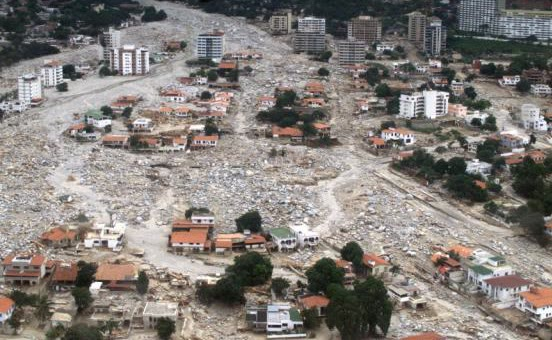
\includegraphics[width=0.62\linewidth]{images/book4/b2-28-caraballeda-debris-flow.jpg}
\par\smallskip{\small Debris-flow deposits on the fan of Caraballeda, on the coast of Venezuela,
after the storm of December 1999: the flows left the main channel and buried the town under
boulders. Photograph: Lawson Smith, U.S. Army Corps of Engineers (public domain).}
\end{omfigure}
% ledger: photo:b2-28-caraballeda, vargas:caraballeda

\section{Tsunamis}\label{sec:b2:geological-hazards:tsunamis}

A tsunami raised by the sudden uplift of the sea floor has a wavelength of tens to hundreds of
kilometres, far more than the depth of the ocean. It is a long wave, and its speed depends only
on the depth.

\begin{proposition}[Long waves]\label{prop:b2:geological-hazards:long-waves}
A surface gravity wave whose wavelength is much larger than the water depth $h$ travels at
$c = \sqrt{gh}$, whatever its wavelength. Where it moves slowly into shallower water without
reflecting or breaking, its amplitude $A$ grows as $h^{-1/4}$.
\end{proposition}

\begin{proof}
The dispersion relation gives the phase speed $c = \omega/k = \sqrt{(g/k)\tanh(kh)}$. For a long
wave $kh = 2\pi h/\lambda \ll 1$, and $\tanh(kh) \approx kh$, so $c = \sqrt{gh}$, independent of
$k$: long waves do not disperse. The energy of the wave per unit area of sea surface is $\frac12
\rho g A^2$, and it travels at $c$. If no energy is reflected or lost, the flux $\frac12\rho g A^2
c$ through any section is the same along the path: $A^2 \sqrt{h}$ is constant, and $A \propto
h^{-1/4}$.
\end{proof}

Over \qty{4000}{m} of water a tsunami travels at \qty{198}{m.s^{-1}}, \qty{713}{km/h}; over
\qty{5000}{m}, \qty{797}{km/h}, the ``more than 800 km/h'' quoted by the warning services. Near the
shore, in \qty{10}{m} of water, it slows to \qty{36}{km/h}; its front is caught up by the water
behind, the wave shortens and steepens, and its height grows.
% ledger: nws:tsunami-speed

\begin{definition}[Tsunami run-up]\label{def:b2:geological-hazards:tsunami}
The \emph{tsunami run-up}\index{tsunami run-up} at a point of the coast is the height, above the
sea level at the time, of the highest ground that the water reaches inland there. The horizontal
distance from the shoreline to that point is the inundation distance.
\end{definition}

Survey teams measure run-ups from water marks, debris lines and damage after each tsunami. The
global tsunami database holds \num{2177} run-up observations for the Indian Ocean tsunami of
26 December 2004, raised by a magnitude 9.1 earthquake off Sumatra, with a maximum water height of
\qty{50.9}{m}, and \num{6429} for the tsunami of 11 March 2011 off Honshu, also of magnitude 9.1,
with a maximum of \qty{39.3}{m}. The two killed \num{227899} and \num{18423} people. In Banda Aceh,
the water reached the middle of the second floor of the mosque below.
% ledger: ncei:tsu-2004, ncei:tsu-2011, usgs:aceh-mosque

\begin{omfigure}
\centering
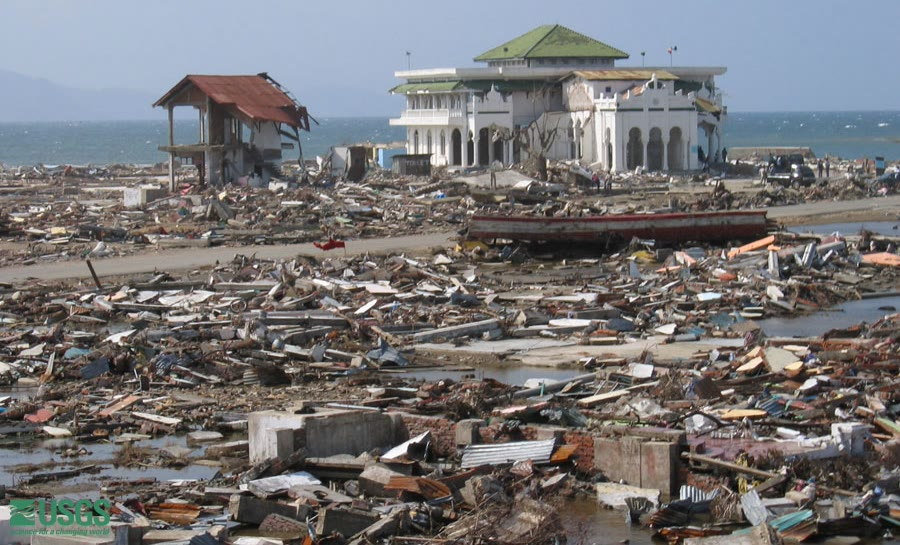
\includegraphics[width=0.62\linewidth]{images/book4/b2-28-aceh-mosque-tsunami.jpg}
\par\smallskip{\small Banda Aceh, Sumatra, on 21 January 2005, after the tsunami of 26 December
2004: a mosque stands amid the rubble of the buildings around it. Photograph: U.S. Geological
Survey (public domain).}
\end{omfigure}
% ledger: photo:b2-28-aceh

\section{Floods}\label{sec:b2:geological-hazards:floods}

\begin{definition}[Flood frequency curve]\label{def:b2:geological-hazards:flood}
The \emph{flood frequency curve}\index{flood frequency curve} of a river at a gauging station is the
curve of the annual peak discharge against its \omterm{def:b2:geological-hazards:return}{return period}, or its annual \omterm{def:b2:geological-hazards:poisson}{exceedance
probability}, built from the station's record of annual peaks and usually extended by a fitted
probability law.
\end{definition}

The rank formula of the school volumes places the points of the curve. It has a reason.

\begin{proposition}[Weibull plotting position]\label{prop:b2:geological-hazards:weibull}
Let $n$ annual peaks be independent and drawn from the same continuous distribution, and let
$G(x)$ be the probability that a year's peak exceeds $x$. The peak of rank $m$, counted from the
largest, has an expected \omterm{def:b2:geological-hazards:poisson}{exceedance probability} $m/(n + 1)$, so that it is plotted at $T = (n +
1)/m$.
\end{proposition}

\begin{proof}
$U = 1 - G(X)$ is uniform on $[0, 1]$ for a continuous law, and $1 - G$ is increasing, so the
$m$-th largest peak corresponds to the $m$-th smallest of $n$ independent uniform variables,
$U_{(m)}$. Its density is $f(u) = \frac{n!}{(m-1)!\,(n-m)!}u^{m-1}(1-u)^{n-m}$: one of the $n$ values
at $u$, $m - 1$ below and $n - m$ above. With the Beta integral $\int_0^1 u^{p}(1-u)^{q}\,\mathrm{d}u
= p!\,q!/(p + q + 1)!$,
\begin{equation*}
\mathbb{E}[U_{(m)}] = \frac{n!}{(m-1)!\,(n-m)!}\cdot\frac{m!\,(n-m)!}{(n+1)!} = \frac{m}{n+1}. \qedhere
\end{equation*}
\end{proof}

The largest peak of a 30-year record is thus plotted at 31 years, and nothing in the record fixes
the 100-year flood. To reach it, the peaks are fitted with a law of extremes, often Gumbel's,
$\Pr(\text{peak} \leq x) = \exp\bigl(-e^{-(x - u)/\alpha}\bigr)$, whose $T$-year flood is $x_T = u
- \alpha\ln\bigl(-\ln(1 - 1/T)\bigr)$: a straight line against $-\ln(-\ln(1 - 1/T))$, extrapolated
beyond the record at a risk that grows with the distance.

\section{Monitoring and early warning}\label{sec:b2:geological-hazards:warning}

\begin{definition}[Early warning system]\label{def:b2:geological-hazards:warning}
An \emph{early warning system}\index{early warning system} is an integrated system of hazard
monitoring, forecasting, risk assessment, communication and preparedness that enables timely
action before a hazardous event. It joins four elements: knowledge of the risk; detection,
monitoring and forecasting of the hazard; the dissemination of warnings; and the preparedness to
respond.
\end{definition}
% ledger: undrr:ews

Physics sets how much time each warning can give. Seismic waves cannot be outrun, but the damaging
S waves travel at about \qty{3.2}{km.s^{-1}} in the upper crust, against \qty{5.8}{km.s^{-1}} for
the P waves: an alert computed from the first P waves recorded near the epicentre reaches a city
before the S waves, by $d(1/3.2 - 1/5.8) = \qty{0.14}{s}$ per kilometre of distance $d$, less the
time to detect and compute. A city \qty{100}{km} away gains at most \qty{14}{s}; near the source a
blind zone gets none (\cref{exo:b2:geological-hazards:12}). A tsunami crossing \qty{100}{km} of sea
\qty{2000}{m} deep takes 12 minutes; across an ocean it takes hours. In 2011, the Japanese
warning was issued about three minutes after the earthquake, but on a magnitude estimated too low,
because the instruments saturated; it was updated with data from an offshore GPS buoy about 28 minutes later.
Deep-ocean pressure recorders, which convert the pressure on the sea floor every 15 seconds into a
sea-surface height, now report passing tsunamis by satellite.
% ledger: data:prem, jma:warning, ndbc:dart
% values: 0.1401 s/km, 14.0 s at 100 km; 140 m/s over 2000 m, 11.9 min per 100 km (calc/ch28.py)

\begin{inthefield}[Watching a slope move]
On a slope known to creep, monitoring teams install instruments that measure the variables of the
infinite-slope equation. Piezometers in boreholes record the pore pressure on the slip surface;
inclinometer tubes, read at depth intervals, show where the ground bends and how fast; GNSS
stations and extensometers record the movement of the surface; a rain gauge records the trigger.
Teams compare the movement with the rain and the water pressure, season after season, and look
for the acceleration that precedes failure.
\end{inthefield}

\section*{Exercises}\label{sec:b2:geological-hazards:exercises}

Data for the exercises, unless stated otherwise: $g = \qty{9.81}{m.s^{-2}}$; unit weight of water
\qty{9.81}{kN.m^{-3}}; the GMPE \eqref{eq:b2:geological-hazards:gmpe} on rock ($G_B = G_C = 0$),
$\sigma = 0.230$; P and S speeds in the upper crust 5.8 and \qty{3.2}{km.s^{-1}}. Round to three
significant figures.
% ledger: bjf93:pga, data:prem

\begin{exercise}[$\star$]\label{exo:b2:geological-hazards:1}
Under the Poisson model: (a) what is the probability of at least one 100-year flood in 30 years?
(b) What is the probability that a century passes without a 100-year flood? (c) Find the \omterm{def:b2:geological-hazards:return}{return
period} of the motion with a \qty{5}{\percent} chance of exceedance in 50 years.
\end{exercise}

\begin{exercise}[$\star$]\label{exo:b2:geological-hazards:2}
Two towns face strong shaking. In town A, it occurs at a rate of once in 200 years and would
destroy \qty{2}{\percent} of its 5000 buildings; in town B, once in 50 years, destroying
\qty{10}{\percent} of its 800 buildings. (a) Find the expected number of buildings destroyed per
year in each town. (b) Which town has the greater risk, though it has the smaller \omterm{def:b2:geological-hazards:risk}{exposure}? (c)
Which of the three factors makes the difference?
\end{exercise}

\begin{exercise}[$\star$]\label{exo:b2:geological-hazards:3}
(a) Find the speed of a tsunami over depths of 4000, 200 and \qty{10}{m}. (b) How long does it
take to cross \qty{1500}{km} of ocean \qty{4000}{m} deep? (c) At what depth would it travel at
\qty{800}{km/h}?
\end{exercise}

\begin{exercise}[$\star$]\label{exo:b2:geological-hazards:4}
A dry, cohesionless sand with $\varphi' = \ang{33}$ forms a long slope. (a) Find its \omterm{def:b2:geological-hazards:slope}{factor of
safety} at \ang{25}. (b) What is the steepest slope it can form? (c) The slope becomes saturated with
the water table at the surface and seepage parallel to it, so that $r_u = \gamma_w\cos^2\beta/\gamma$
with $\gamma = \qty{20}{kN.m^{-3}}$. Show that $F = (1 - \gamma_w/\gamma)\tan\varphi'/\tan\beta$ and
compute it at \ang{25}.
\end{exercise}

\begin{exercise}[$\star\star$]\label{exo:b2:geological-hazards:5}
The global catalogue holds 696 earthquakes of magnitude at least 7 in the 50 years 1976--2025, and
the mean interval between them is 26.2 days. (a) Find their mean annual rate. (b) Under the
Poisson model, what is the probability that 30 days pass without one? Compare with the observed
fraction of intervals longer than 30 days, 0.304. (c) What is the probability of at least one in a
given week?
\end{exercise}

\begin{exercise}[$\star\star$]\label{exo:b2:geological-hazards:6}
(a) Find the median PGA of a magnitude 6.5 earthquake on rock at $d = 0$, 10, 30 and
\qty{100}{km}. (b) What would it be at \qty{10}{km} on a class C site? (c) Between which values
does the PGA on rock at \qty{10}{km} lie with a probability of about \qty{68}{\percent}?
\end{exercise}

\begin{exercise}[$\star\star$]\label{exo:b2:geological-hazards:7}
A river's annual peaks over 12 years were, in \unit{m^3.s^{-1}}: 212, 148, 305, 176, 251, 133, 188,
420, 160, 229, 195, 268. (a) Give the \omterm{def:b2:geological-hazards:return}{return periods} of the four largest. (b) Estimate the 10-year
flood by interpolating linearly in $\ln T$ between the two largest. (c) Why can this record say
nothing reliable about the 100-year flood?
\end{exercise}

\begin{exercise}[$\star\star$]\label{exo:b2:geological-hazards:8}
At a restless volcano the observatory estimates: unrest magmatic 0.6; eruption if magmatic 0.4;
explosive if eruption 0.5; a \omterm{def:b2:eruptive-styles:pdc}{pyroclastic flow} reaching a given valley if explosive 0.3. (a) Find
the probability of a \omterm{def:b2:eruptive-styles:pdc}{pyroclastic flow} in the valley. (b) Find the probability of an eruption, and
of an eruption without a flow in the valley. (c) New deformation data raise the probability of an
eruption, if the unrest is magmatic, to 0.7. Update (a).
\end{exercise}

\begin{exercise}[$\star\star$]\label{exo:b2:geological-hazards:9}
A dry soil with $c' = \qty{8}{kPa}$, $\varphi' = \ang{30}$ and $\gamma = \qty{19}{kN.m^{-3}}$ lies on
a \ang{35} slope. (a) Find the thickness $z_c$ at which $F = 1$. (b) Find $F$ for a layer
\qty{2}{m} thick. (c) The same layer becomes saturated, with the water table at the surface and
$r_u = \gamma_w\cos^2\beta/\gamma$. Find $F$.
\end{exercise}

\begin{exercise}[$\star\star\star$]\label{exo:b2:geological-hazards:10}
(a) Show that the Poisson model is memoryless: the probability of no event in $[s, s + t]$, given
none in $[0, s]$, is $e^{-t/T}$, whatever $s$. (b) A fault has a \omterm{def:b2:geological-hazards:return}{return period} of 475 years for its
large earthquakes and has had none for 400 years. What is, under the model, the probability of one
in the next 50 years? (c) The elastic rebound of the Year 1 volume suggests that the probability
should instead grow with the time since the last earthquake. Which assumption of the Poisson model
does it contradict, and why do hazard maps keep the model for areal sources?
\end{exercise}

\begin{exercise}[$\star\star\star$]\label{exo:b2:geological-hazards:11}
A tsunami of amplitude \qty{0.5}{m} and period 20 minutes crosses an ocean \qty{4000}{m} deep. (a)
Using the energy-flux argument of the proposition on long waves, find its amplitude in \qty{10}{m}
of water. (b) Find its wavelength at both depths. (c) Give two reasons why the run-up at the coast
can differ greatly from this estimate.
\end{exercise}

\begin{exercise}[$\star\star\star$]\label{exo:b2:geological-hazards:12}
An earthquake \omterm{def:b2:geological-hazards:warning}{early warning system} issues an alert 4 seconds after the P wave reaches its station
nearest to the epicentre, \qty{10}{km} away. Neglect the depth of the source. (a) When is the
alert issued after the earthquake? (b) How many seconds before the S wave does a town \qty{50}{km}
from the epicentre receive it? A town at \qty{100}{km}? (c) Find the radius of the blind zone, where
the S wave arrives before the alert.
\end{exercise}

\begin{problem}[{Weekend problem --- A town between a fault and a slope}]\label{pb:b2:geological-hazards:1}
A town on rock lies \qty{10}{km} from a source zone; all its earthquakes are taken at
$d = \qty{10}{km}$. Their recurrence is $\log_{10} N(\geq M) = 4.0 - 1.0\,M$ per year for $M \geq 5$,
truncated at $M_{\max} = 7.5$. The shaking follows the GMPE \eqref{eq:b2:geological-hazards:gmpe}
with $\sigma = 0.230$. Above the town, a soil layer \qty{3}{m} thick rests on a \ang{30} slope,
with $\gamma = \qty{19}{kN.m^{-3}}$, $c' = \qty{4}{kPa}$ and $\varphi' = \ang{34}$; water has unit
weight \qty{9.81}{kN.m^{-3}}. Round to three significant figures.

\noindent\textbf{Part I --- Recurrence.}
\begin{enumerate}
  \item Find the annual rates of earthquakes of magnitude at least 5, 6 and 7, ignoring the
        truncation.
  \item Give the corresponding \omterm{def:b2:geological-hazards:return}{return periods}.
  \item With the truncation, find the rate of earthquakes above 7.5, and the rate of those between 7
        and 7.5.
  \item Find the rates of the magnitude bins 5--6 and 6--7.
  \item What is the probability of at least one earthquake of magnitude 6 or more in 50 years?
  \item And of magnitude 7 or more?
\end{enumerate}

\noindent\textbf{Part II --- Ground motion at the town.}
\begin{enumerate}[resume]
  \item Find $r$, and the distance term $-0.778\log_{10} r$.
  \item Represent the three bins by the magnitudes 5.5, 6.5 and 7.25. Find the median
        $\log_{10}\mathrm{PGA}$ and the median PGA of each.
  \item Find the PGA exceeded with a probability of \qty{16}{\percent} by a magnitude 6.5.
  \item What is the probability that a magnitude 6.5 produces more than \qty{0.3}{g}?
  \item What is the median PGA of the largest possible earthquake?
\end{enumerate}

\noindent\textbf{Part III --- The hazard curve.}
\begin{enumerate}[resume]
  \item Find the annual rate of exceedance of \qty{0.2}{g}, summed over the three bins.
  \item The same for \qty{0.3}{g}.
  \item The same for \qty{0.4}{g}.
  \item What annual rate corresponds to \qty{10}{\percent} in 50 years?
  \item Between which two of the three levels does that rate fall?
  \item Interpolating linearly in $\ln\lambda$ against $\ln a$, find the PGA with a
        \qty{10}{\percent} chance of exceedance in 50 years.
  \item Which bins contribute most to the rate at \qty{0.3}{g}? Comment, using the answer to
        question~11.
\end{enumerate}

\noindent\textbf{Part IV --- The slope above the town.}
\begin{enumerate}[resume]
  \item Find the \omterm{def:b2:geological-hazards:slope}{factor of safety} of the dry slope.
  \item Find it when the layer is saturated, the water table at the surface ($r_u =
        \gamma_w\cos^2\beta/\gamma$).
  \item Up to what fraction of the layer's thickness can the water table rise before the slope fails?
  \item In a pseudo-static analysis (admitted), shaking adds a horizontal force $kW$. Find the
        critical $k$ of the dry slope, at which $F = 1$.
  \item Taking $k$ equal to the PGA in units of $g$, which magnitude produces the critical value as
        its median at the town? Compare with the answer to question~17.
  \item To sum up: what is the \omterm{def:b2:geological-hazards:psha}{peak ground acceleration} with a \qty{10}{\percent} chance of being
        exceeded in 50 years at the town?
\end{enumerate}
\end{problem}
